%\setcounter{chapter}{1}
\pagenumbering{arabic}
\setcounter{page}{1}

\titleformat{\chapter}[display]{\normalfont\LARGE\bfseries}{}{1em}{\thechapter.~}
\chapter{Laboratorio: Programación en Arduino.}


\section{Objetivos}
Este es un laboratorio introductorio que busca:
\begin{itemize}
	{\small \item Compilar y cargar  un programa en Arduino.
	\item Configurar los pines del microcontrolador.
	\item Estudiar la tabla ASCII generada con el Arduino.
	\item Estudiar la crecación de funciones lógicas: AND, OR, XOR, NAND, NOR.
	\item Estudiar la cuantizacion de una señal. }
\end{itemize} 


\section{Equipos y materiales}
Para este laboratorio de necesitaran:
\begin{itemize}
	{\small \item 1 Arduino UNO o equivalente: MEGA o ESP32.
	\item 1 Multímetro.
	\item 5 Resistencias de 270 o 330 $\Omega$.
	\item 2 Resistencias de 1k$\Omega$.
	\item 2 interruptores pulsadores.
	\item 1 Protoboard.
	\item 5 Diodes emisor de luz (LEDs).
	\item 2 Generadores de funciones.
	\item 2 Osciloscopio.
	\item 1 Computadora portátil.}
\end{itemize}

\section{Marco de referencia}

Un micro-controlador es un circuito integrado pequeño que contiene un microprocesador, memoria y periféricos como entradas/salidas (IO), comunicación, almacenamiento y sensores. Estos componentes están integrados en un solo chip y pueden ser programados para controlar diferentes dispositivos y sistemas.

Entre las partes que pueden contener los micro-controladores se encuentran: Microprocesador: es la unidad aritmética lógica,  registros asociados y controladores  que realizan  las operaciones del sistema y es responsable de ejecutar las instrucciones del programa.
Memoria: donde se almacena el programa y los datos.
Entradas/Salidas (IO): permite la comunicación entre el micro-controlador y el mundo exterior.
Comunicación: permite que el micro-controlador se comunique con otros dispositivos a través de diferentes protocolos como USB, Ethernet, etc.
Almacenamiento: permite almacenar datos en el dispositivo, como una EEPROM o una memoria flash.
Sensores: permiten medir diferentes variables ambientales como la temperatura, la humedad, la presión, etc.

Los micro-controladores tienen muchos usos, incluyendo: Control de motores,
Automatización de procesos industriales,
Dispositivos de medida y monitoreo,
Control de sistemas de iluminación y calefacción,
Control de sistemas de seguridad,
Control de electrodomésticos y dispositivos de consumo,
Control de sistemas de comunicación,
Control de sistemas de vehículos,
Control de robots y sistemas automatizados.

\subsection{Arduino}

El Arduino es una plataforma de desarrollo de hardware y software libre basada en un micro-controlador. La programación de Arduino se basa en el lenguaje de programación C++ y utiliza un entorno de desarrollo integrado (IDE) específico llamado Arduino IDE. El Arduino IDE es una aplicación de escritorio que se utiliza para escribir, depurar y cargar código en el micro-controlador.

El procedimiento básico de programación del Arduino es el siguiente:

\begin{enumerate}
	\item Conectar el Arduino a la computadora mediante un cable USB.
	\item Abrir el Arduino IDE y seleccionar el tipo de Arduino y la tarjeta que se va a utilizar en el menú Herramientas.
	\item Escribir el código en el editor de código del Arduino IDE, utilizando el lenguaje de programación C++.
	\item Verificar el código compilando el código utilizando el botón verde de compilación del Arduino IDE.
	\item Cargar el código en el Arduino utilizando el botón azul de carga del Arduino IDE.
	\item Observar el comportamiento del código en los pines de entrada y salida del Arduino, si es necesario realizar cambios en el código para obtener el resultado deseado.
	\item Repetir los pasos 3-6 hasta que el código funcione correctamente.

\end{enumerate}

El esquema básico de programación de Arduino utiliza dos funciones esenciales \cite{Margolis20}: setup() y loop().

La función \href{https://www.arduino.cc/reference/en/language/structure/sketch/setup/}{setup()}: Es la primera función que se ejecuta cuando el Arduino se enciende o se reinicia. En esta función se configuran los pines de entrada y salida, se establecen las velocidades de comunicación, se inicializan las variables, entre otras tareas de configuración. 

La función \href{https://www.arduino.cc/reference/en/language/structure/sketch/loop/}{loop()}: Es la función que se ejecuta continuamente después de que se ha ejecutado la función setup(). En esta función se escriben las instrucciones que se deben ejecutar continuamente, como la lectura de sensores, el control de actuadores, la comunicación con otros dispositivos, entre otras tareas.

Las instrucciones y funciones del lenguaje C++ para Arduino pueden ser consultadas en el \href{https://www.arduino.cc/reference/en/}{siguiente vínculo}.

\section{Metodología}

Este laboratorio tiene una duración de 4 lecciones, repartidas en dos semanas. Los estudiantes deben mostrar durante las clases programadas las tres actividades propuestas. Deben recabar fotografías y resultados de los equipos de medición para elaborar las evidencias. Las evidencias se subirán al TecDigital la semana siguiente finalizadas las actividades.

\section{Práctica en Clase}

\subsection{Actividad 1}
Los símbolos  para impresión \href{https://es.wikipedia.org/wiki/ASCII}{ASCII} (\textit{American Standard Code for Information Interchange}) es una codificación de distintos símbolos a un valor numérico que usualmente es mostrado en decimal, binario o hexagecimal.

El siguiente programa muestra la tabla ASCII no extendida que genera el Arduino. Dicho programa imprime en el puerto serial el numero decimal, su equivalente binario y hexagecimal y el simbolo respectivo. Por ejemplo el símbolo !, equivale a 33 en sistema decimal, a 21 en hexagecimal, a 41 en octal,y a 100001 en binario. El código de este proyecto lo puede copiar del enlace: \href{https://docs.arduino.cc/built-in-examples/communication/ASCIITable}{Tabla ASCII}.
 
\subsubsection{Conteste las preguntas:}
¿El símbolo ASCII ! esta bien representado en decimal?
¿Cual es la diferencia del comando serial.write y serial.print()?
¿Corrobore si las conversiones entre decimal, octal y hexagecimal son correctas?


\subsection{Actividad 2}
El  código del apéndice \ref{ApendiceA} apaga y enciende un LED según el estado de un botón. La figura \ref{fig:fig1} muestra el esquema básico de conexión.

Elimine el botón y alimente el Arduino con un generador de funciones que brinde una señal cuadrada de 0 a 5 voltios. Conecte los dos canales del osciloscopio en la  entra y salida. Recuerde que todas las tierras deben estar conectadas entre si. 

\subsubsection{Conteste las preguntas:}
¿Cuanto es el retardo de la señal?
¿Cual es la frecuencia de la señal de entrada en que la señal de salida se distorsiona? Es decir, la señal de salida no es  inversa a la señal de entrada. Recuerde capturar las pantallas del osciloscopio en ambos casos.

\begin{figure}[H]
	\centering
	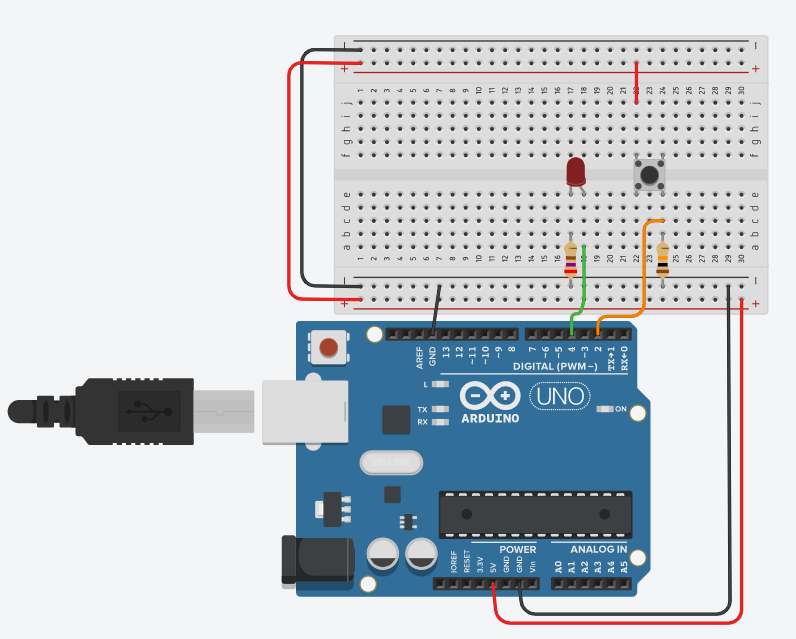
\includegraphics[width=0.5\linewidth]{Imagenes/Fig1}
	\caption{Diagrama de conexón del botón y LED.}
	\label{fig:fig1}
\end{figure}


\subsection{Actividad 3}

Esta actividad permite analizar el comportamiento de las conectivas lógicas  AND, OR, XOR, NAND, y NOT, y exportar los resultados al puerto serial, así como mostrar los resultados mediante los LEDs conectados a los pines $\left\lbrace4, 5, 6, 7, 8 \right\rbrace$ ; el código de ejemplo se muestra en el apéndice \ref{ApendiceB}. Las entradas declaradas mediante los pines $\left\lbrace2, 3 \right\rbrace$ reciben las señales de dos generadores de funciones. Los generadores brindan una señal triangular que oscila ente $[0-5]$ voltios, debe ajustar cuidadosamente con el osciloscopio cada señal. La señal del pin 2 tendrá una frecuencia del doble del pin 3. Adicionalmente las señales  triangulares alimentaran el convertidor Analógico-Digital (ADC) mediante los pines A0 y A1. Conecte su Arduino según el esquema de la Figura \ref{fig:fig2}.  Imprima los resultados en el puerto serial, ajuste la velocidad del puerto con valores de: \{ 9600, 14400, 19200, 28800, 38400, 57600\}bps según la frecuencia seleccionada del generador de funciones.

\begin{figure}[H]
	\centering
	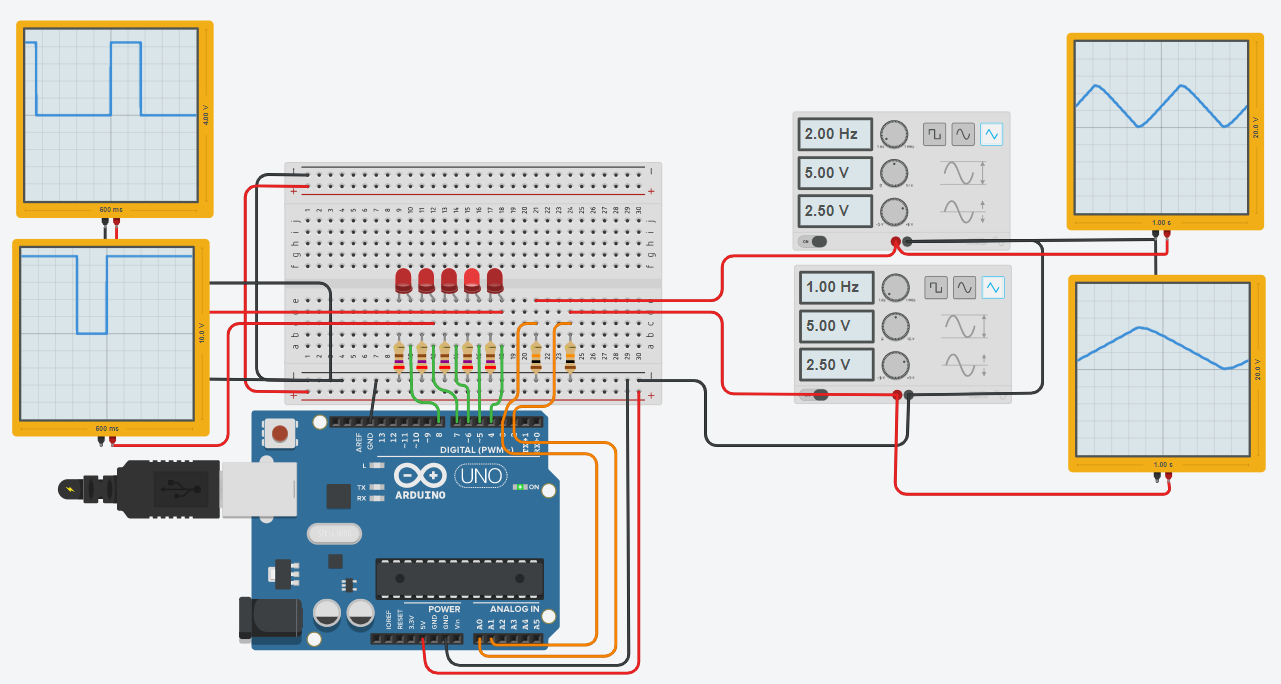
\includegraphics[width=0.8\linewidth]{Imagenes/Fig2}
	\caption{Esquema de conexión del Arduino, Generador de funciones y Osciloscopio}
	\label{fig:fig2}
\end{figure}


El código del Anexo B implementa las funciones lógicas AND, OR. Un repaso de como implementar funciones en C se muestra en \href{https://aprendiendoarduino.wordpress.com/2016/11/16/funciones-definidas-por-usuario-2/}{este enlace.} 

\subsubsection{Conteste las preguntas:}

Guarde los datos del puerto serial en un archivo .TXT e importelos en MS EXCEL para graficar los datos.
Se recomienda utilizar el monitor serial de MS CODE STUDIO dado que este permite salvar los datos.
¿Se logra apreciar las señales triangulares y digitales?
¿Las gráficas de las señales digitales de entrada y salida cumplen las tablas de verdad de las conectivas lógicas?
¿Cual es el voltaje de entrada en bajo máximo $V_{IL} max$?,
¿Cual es el voltaje de entrada en alto mínimo $V_{IH} min$?,
¿Cual es el error que presenta las mediciones de los voltajes ?,
¿Si desea un error de $\pm1$ mV, de cuantos bits debe ser el ADC?¿Explique?

\section*{Apéndices}
\setcounter{chapter}{1}
\setcounter{section}{5}
\section{Código actividad 2}
\label{ApendiceA}
{\scriptsize 
	
	\begin{lstlisting}[language=C++]
	/*
	Instituto Tecnológico de Costa Rica
	LAB #1 de Laboratorio de Control Eléctrico.
	Fecha: 25/01/2023
	Ing. Luis D. Murillo
	
	Este programa apaga el LED cuando se presiona el botón. 
	
	*/
	// Declaracione de entradas y salidas
	const int BUTTON =2;  // Boton conectado al pin 2
	const int LED =4;     // LED conectado al pin 4
	
	// CONFIGURACION DE ENTRADAS Y SALIDAS
	void setup() {
		pinMode(LED, OUTPUT);    // configuramos el pin del LED como salida
		digitalWrite(LED, HIGH);  // Encendemos el LED
		pinMode(BUTTON, INPUT);  // configuramos el pin del botón como entrada
	}
	// PROGRAMA PRINCIPAL
	void loop() {
		bool buttonState = digitalRead(BUTTON);  // leemos el estado del botón
		if (buttonState == HIGH) {
			digitalWrite(LED, LOW);  // apagamos el LED
		} else {
			digitalWrite(LED, HIGH);   // encendemos el LED
		}
	}
	
	\end{lstlisting}
	
}

\section{Código actividad 3}
\label{ApendiceB}
{\scriptsize 
		
	\begin{lstlisting}[language=C++]
		 /*
		Instituto Tecnológico de Costa Rica
		Laboratorio de Control Eléctrico.
		Lab #1: Conectiva logicas y señal analógica
		Fecha: 24/01/2023
		Ing. Luis D. Murillo
		
		Implementación de Funciones Lógicas AND, OR, XOR, NAND, NOR de 2 entradas
		*/
		// Declaracione de constantes
			const int PinEntrada[2]={2,3};
			const int PinSalidas[5]={4,5,6,7,8};
			const int PinAnalogico[2] = {A0, A1};
			int ValorAnalojLeido[2]={0,0};
			float ValorVoltage[2]={0.0,0.0};
			boolean Mapa_entradas[2];
			boolean ResultadoLogico[5]={false, false, false, false, false};
		
		// Configuracion de Pines de entrada y salida
		void setup(){
			Serial.begin(9600);
			Serial.println("-----");
			Serial.println((sizeof(PinEntrada)/2));
			Serial.println((sizeof(PinSalidas)/2));
			Serial.println("-----");
		
		// Initializa los pines:
		for (int i = 0; i < (sizeof(PinSalidas)/2); i++) {
			if (i<(sizeof(PinEntrada)/2)) {
				pinMode( PinEntrada[i], INPUT);
			}
			pinMode(PinSalidas[i], OUTPUT);
			}
		delay(2);
		}
		
		void loop()
		{		
			//LECTURA DE LAS ENTRADAS Y SALIDAS 	
			for(int i=0; i<(sizeof(PinSalidas)/2);i++){
				if(i<(sizeof(PinEntrada)/2)){
					// Lectura de entradas digitales
					Mapa_entradas[i]=digitalRead(PinEntrada[i]);
					// Lectura de los valores analógicos
					ValorAnalojLeido[i] = analogRead(PinAnalogico[i]);
					// Funcion de mapeo :
				ValorVoltage[i]= (map(ValorAnalojLeido[i], 0, 1023, 0, 500)/100.0);
				}
			// Escritura de salida digital
			digitalWrite(PinSalidas[i],ResultadoLogico[i]);
			}
		
		//EJECUCION DEL PROGRAMA
			ResultadoLogico[0]=AND(Mapa_entradas[1],Mapa_entradas[0]);
			ResultadoLogico[1]=OR(Mapa_entradas[1],Mapa_entradas[0]);
			ResultadoLogico[2]=XOR(Mapa_entradas[1],Mapa_entradas[0]);
			ResultadoLogico[3]=NAND(Mapa_entradas[1],Mapa_entradas[0]);
			ResultadoLogico[4]=NOR(Mapa_entradas[1],Mapa_entradas[0]);
		
		//IMPRESION DE RESULTADOS ENTRADA Y SALIDAS
		
			Serial.print(Mapa_entradas[0]);
			Serial.print(", ");
			Serial.print(ValorVoltage[0]);
			Serial.print(", ");
			Serial.print(Mapa_entradas[1]);
			Serial.print(", ");
			Serial.print(ValorVoltage[1]);
			Serial.print(", ");
			Serial.println(ResultadoLogico[0]);
			Serial.print(", ");
			Serial.print(ResultadoLogico[1]);
			Serial.print(", ");
			Serial.print(ResultadoLogico[2]);
			Serial.print(", ");
			Serial.print(ResultadoLogico[3]);
			Serial.print(", ");
			Serial.println(ResultadoLogico[4]);
		}
		
		//DEFINICION DE LAS FUNCIONES LÓGICAS
		// Forma de programacion Booleana
		bool AND (bool X, bool Y ){
		return (X && Y ); 
		}
		
		// Forma de programacion con estructuras de control
		bool OR (boolean X, bool Y ){
		if (X || Y) {return true;} 
		else {return false;}
		}
		
		// Completar código
		bool XOR (bool X, bool Y ){
				; 
		}
		
		bool NAND (bool X, bool Y ){
				; 
		}		
		
		bool NOR (bool X, bool Y ){
				; 
		}
		\end{lstlisting}
}

